%
%
%
%

\documentclass{article}
         
\usepackage{graphicx,xcolor}
\usepackage[load-headings]{exsheets}

\usepackage[frenchb]{babel}
\usepackage{amsmath,amssymb,bm}
\usepackage{enumitem}
\usepackage{lmodern,microtype}
\usepackage[a4paper,left=4cm]{geometry}
\usepackage{tikz}
\usepackage{hyperref}
\usetikzlibrary{arrows,decorations,calc}
\usetikzlibrary{decorations.pathmorphing,patterns,decorations.pathreplacing,decorations.markings}


\usepgflibrary{arrows}



\newcommand{\diff}{\text{d}}
\renewcommand{\i}{\text{i}}
\renewcommand{\Re}{\mathop{\text{Re}}}



\begin{document}
\noindent
{\textsc{Universit\'e catholique de Louvain}} \hfill \'Ecole de Physique\\
Facult\'e des Sciences \hfill 5 December 2024\\
\hrule

\bigskip

\begin{center}
  \textbf{LPHYS2114 Non Linear Dynamics}\\
  \textbf{S\'erie 10 -- Tent map. Linear 1d maps}
\end{center}

\SetupExSheets{headings=runin-fixed-nr}


\subsection*{Tent map and the Cantor set}

\noindent We will consider the tent map defined by:
  \begin{equation}
    f(x) =
    \begin{cases}
      3x, &  x \leqslant 1/2,\\
      3(1-x), & x \geqslant 1/2.
    \end{cases}
    \label{eqn:Tent}
  \end{equation}
   The graph of $f$ is shown in Figure \ref{fig:Tent}. We are interested in the collection of points $x_0$ from which orbits originate.
   
   
   \begin{figure}[h]
   \centering
   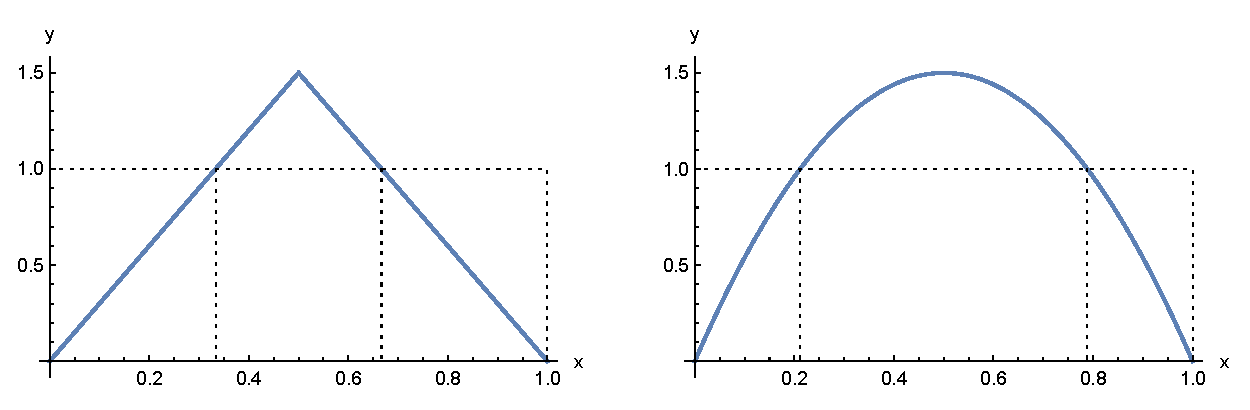
\includegraphics[width=\textwidth]{LogisticTent}
   \caption{\textit{Left:} Graph of the tent map defined by \eqref{eqn:Tent}. \textit{Right:} Graph of the logistic map with $a=6$.}
   \label{fig:Tent}
   \end{figure}
   
   \begin{question}\textbf{Cantor set $\bm {1/3}$.}
     It is convenient to introduce the Cantor set $1/3$. To define it we consider the interval $[a,b]$ and a function $T$ defined by
   \begin{equation}
     T([a,b]) = [a,a+(b-a)/3]\cup [b-(b-a)/3,b].
   \end{equation}
    For the union of disjoint intervals $I = \bigcup_{k=1}^n[a_k,b_k]$, we define $T(\bigcup_{k=1}^n[a_k,b_k]) = \bigcup_{k=1}^nT([a_k,b_k])$, i.e. $T$ agit s\'epar\'ement sur chaque intervalle de l'union.
   
   
   \begin{enumerate}[label=(\alph*)]
     \item Given $K_0=[0,1]$. We iteratively define $K_{n+1} = T(K_n),\,n\geqslant 0$. Calculate $K_1,K_2,K_3$ and the et les tracer.
     \item The Cantor set is $K_\infty = \lim_{n\to \infty}K_n$. Show that this collection is not empty.
     \item Show that the sum $|K_n|$ of the length of the intervals of $K_n$ is given by $|K_n|=(2/3)^n$. Deduce that $K_\infty$ is the null measure.
   \end{enumerate}
    The ternary representation of a point $x\in K_0$ is given by
     \begin{equation}
       x = .a_1a_2a_3\dots = \sum_{n=1}^\infty \frac{a_n}{3^n}, \quad a_n \in \{0,1,2\}.
     \end{equation}
     On admet toutes les suites de chiffres ternaires, ce qui implique que la repr\'esentation n'est pas unique. En effet pour $a_n>0$ on a $.a_1\dots a_n\bar 0=.a_1\dots (a_n-1)\bar 2$.
   \begin{enumerate}[label=(\alph*),resume]
     \item Montrer que $K_\infty = \{x=.a_1a_2a_3\dots | a_n \in\{0,2\},\, n\geqslant 0\}$. En d\'eduire que $K_\infty$ n'est pas d\'enombrable.
        \item \'Etablir que l'application $x\mapsto 3x$ est une bijection entre $[0,1/3]\cap K_\infty$ et $K_\infty$. Expliquer dans quel sens il est alors autosimilaire.

        \end{enumerate}
   \end{question}
  
   \begin{question}\textbf{Tent map.} We now use the results from the previous question to study the tent map $f$.
  
  \begin{enumerate}[label=(\alph*),resume]
     \item Prove that the orbit of points $x_0\notin K_0=[0,1]$ under the map  $f$ is not n'est pas born\'ee.
     \item Show that the points $x_0\in K_0\backslash K_1$ leave $K_0$ after one iteration. Deduce that all the orbits are not En d\'eduire que leur orbite n'est pas born\'ee.
     
     \item Find all points which leave the set $K_0$ after $n$ iterations.
     
     \item Show taht the set of points Montrer que l'ensemble des points dont l'orbite reste dans $K_0$ est $K_\infty$. Conclure.
          
  \end{enumerate}
     \end{question}
     
\begin{question}
\textbf{L'application logistique avec $\bm{a>4}$.} We now will look at the logistic map with $a>4$, shown in Figure \eqref{eqn:Tent} and the et de l'\'etude de l'application en tente, d\'ecrire l'ensemble des points $x_0$ dont l'orbite est born\'ee.
\end{question}

\subsection*{Linear iterations in the plane}

\begin{question}
  \textbf{A map on the plane.} We consider the linear map $f:\mathbb R^2 \to \mathbb R^2$ defined by $f(\bm x) = A\bm x$ with
  \begin{equation}
    A =
    \begin{pmatrix}
      2 & 1\\
      1 & 1
    \end{pmatrix}.
  \end{equation}
  \begin{enumerate}[label=(\alph*)]
    \item Calculate the eigan-values and eigan-vectors of $A$.
    \item Deduce the phase portrait of the map $\bm x_{n+1} = f(\bm x_n),\, n\geqslant 0$.
  \end{enumerate}
\end{question}

\begin{question}
  \textbf{Conserved Quantities.}
  A function $E:\mathbb R^m \to R$ is called quantity conserving for the map $f:\mathbb R^m \to \mathbb R^m$ if $E\circ f = E$.  
  
  
    \begin{enumerate}[label=(\alph*)]
    \item Show that $E$ is est constante le long les orbites de l'it\'eration $\bm x_{n+1} = f(\bm x_n)$ d\'efinie par $f$.

    \item On consid\`ere l'application lin\'eaire $f(\bm x) = A \bm x$ avec $\bm x\in\mathbb R^2$. Show that $E(\bm x) = x_1^2+x_2^2$ is quantity conserving for
    \begin{equation}
      A = \begin{pmatrix}
        0 & 1\\
        -1 & 0
      \end{pmatrix}.
    \end{equation}
    \item Sketch the phase portrait of the map defined by $f$.
    \item Find the non-trivial conserved quantities for 
    \begin{equation}
      A = \begin{pmatrix}
        0 & 1\\
        1 & 0
      \end{pmatrix}
      \quad 
      \text{et}
      \quad
      A = \begin{pmatrix}
        2 & 0\\
        0 & 1/3
      \end{pmatrix}.
    \end{equation}
  \end{enumerate}
\end{question}


\end{document}

